\documentclass[12pt]{article} \usepackage[utf8]{inputenc}
\usepackage{bbm}
\usepackage{scrextend, layout, bm  }
\usepackage{fancyhdr,graphicx}
\usepackage[margin=1in]{geometry}
\usepackage{listings}
\pagenumbering{gobble}
\usepackage{amsmath, amssymb}
\DeclareMathOperator{\U}{\mathbb{U}}
\DeclareMathOperator{\G}{\mathbb{G}}
\DeclareMathOperator{\Tau}{\mathcal{T}}
\DeclareMathOperator{\A}{\mathcal{A}}
\DeclareMathOperator{\prob}{\mathbb{P}}
\DeclareMathOperator{\RR}{\mathbb{R}}
\DeclareMathOperator{\ind}{\mathbbm{1}}
\DeclareMathOperator{\convprob}{\stackrel{\prob}{\rightarrow}}
\DeclareMathOperator{\convw}{\stackrel{w}{\rightarrow}}
\renewcommand{\vec}[1]{\mathbf{#1}}
\usepackage{enumitem}
\pagestyle{plain}% Set page style to plain.
\setlength{\headsep}{5pt}

\begin{document}
\noindent Greg Benton, gwb67\\
CS 6241\\
Homework 2\\

\subsection*{Spectral Clustering Methods}

For this homework I implemented spectral clustering algorithms for clustering nodes of a connected graph into arbitrary numbers of clusters. Following the lecture notes, and the tutorial provided in \cite{tutorial}, we consider two objective functions for finding optimal ways of cutting an arbitrary undirected, positively weighted graph into $k$ clusters: Ratio cut, and Ncut. Just to set up notation, we define $A_i$ as the $i^{th}$ cluster from graph $A$, the total of the weights in $A_i$ as $\text{vol}(A)$, and $\bar{A}_i$ as the complement of $A_i$. The `cut' of two clusters is the sum of the weights of edges between them.

Ratio cut seeks to minimize the cost of the following,
$$
  RC(A_1, \dots, A_k) = \frac{1}{2}\sum_{i=1}^{k}\frac{\text{cut}(A_i, \bar{A}_i)}{|A_i|}.
$$
Ncut seeks to minimize
$$
  NC(A_1, \dots, A_k) = \frac{1}{2}\sum_{i=1}^{k}\frac{\text{cut}(A_i, \bar{A}_i)}{\text{vol}(A_i)}.
$$

I will skip over the derivation here, but it was show in class and is given a good treatment in \cite{tutorial} that approximate solutions to the Ratio cut problem can be found by performing k-means clustering on the first $k$ eigenvalues of the graph Laplacian. Likewise an approximate solution to the Ncut problem can be found by performing $k$-means clustering on the first $k$ eigenvalues of the \textit{normalized} graph laplacian, $L = D - W$. Note, $W$ is the weighted adjacency matrix of the graph, and $D$ is a diagonal matrix where $d_i$ is the out degree of the $i^{th}$ node.

So for Ratio cut, at the highest level, we do the following:
\begin{enumerate}[label=(\arabic*)]
  \item Compute $L = D - W$
  \item Compute the first $k$ eigenvectors of $L$ as columns of matrix $U$.
  \item Using rows of $U$ as observations in $\mathbb{R}^k$, perform $k$-means clustering to return clusters $C_1, \dots, C_k$.
\end{enumerate}

For Ncut we proceed similarly with a couple minor modifications:
\begin{enumerate}[label=(\arabic*)]
  \item Compute $L = D - W$
  \item Normalize $L = D^{-1/2}L D^{-1/2}$
  \item Compute the first $k$ eigenvectors of $L$ as columns of matrix $U$
  \item Normalize $U = D^{-1/2}U$
  \item Using rows of $U$ as observations in $\mathbb{R}^k$, perform $k$-means clustering to return clusters $C_1, \dots, C_k$.
\end{enumerate}


\subsubsection*{$K$-Means}

One of the components of this formulation is the use of $k$-means clustering. Just to round out the homework I implemented this algorithm from scratch (code included below). A high-level overview of the algorithm is:
\begin{enumerate}[label=(\arabic*)]
  \setcounter{enumi}{-1}
  \item Start with $n$ nodes to be sorted into $k$ clusters
  \item Randomly initialize $k$ centers of the clusters:
  \item Until convergence or for a fixed number of iterations:
  \begin{enumerate}[label=(\roman*)]
    \item Assign each node to the nearest cluster
    \item Re-center each cluster to the geometric center of it's assigned nodes
  \end{enumerate}
  \item return the node assignments and clusters.
\end{enumerate}

\subsection*{Star Wars Co-Appearance Network}

To test these algorithms I chose to apply them to a network consisting of co-appearances of Star Wars characters \cite{star-wars}. A word of warning, this assumes at least a cursory knowledge of Star Wars just in terms of who the major characters are and where they appear in the saga. The nodes in this graph represent 110 characters from the Star Wars movies (Episodes 1-7), where edges are present when two characters have appeared on screen together, and the weight of the edge represents the number of times they co-appear.
Figure \ref{fig: graph} shows what the graph looks like for the first 6 episodes, taken from \cite{star-wars}.

\begin{figure}
    \centering
    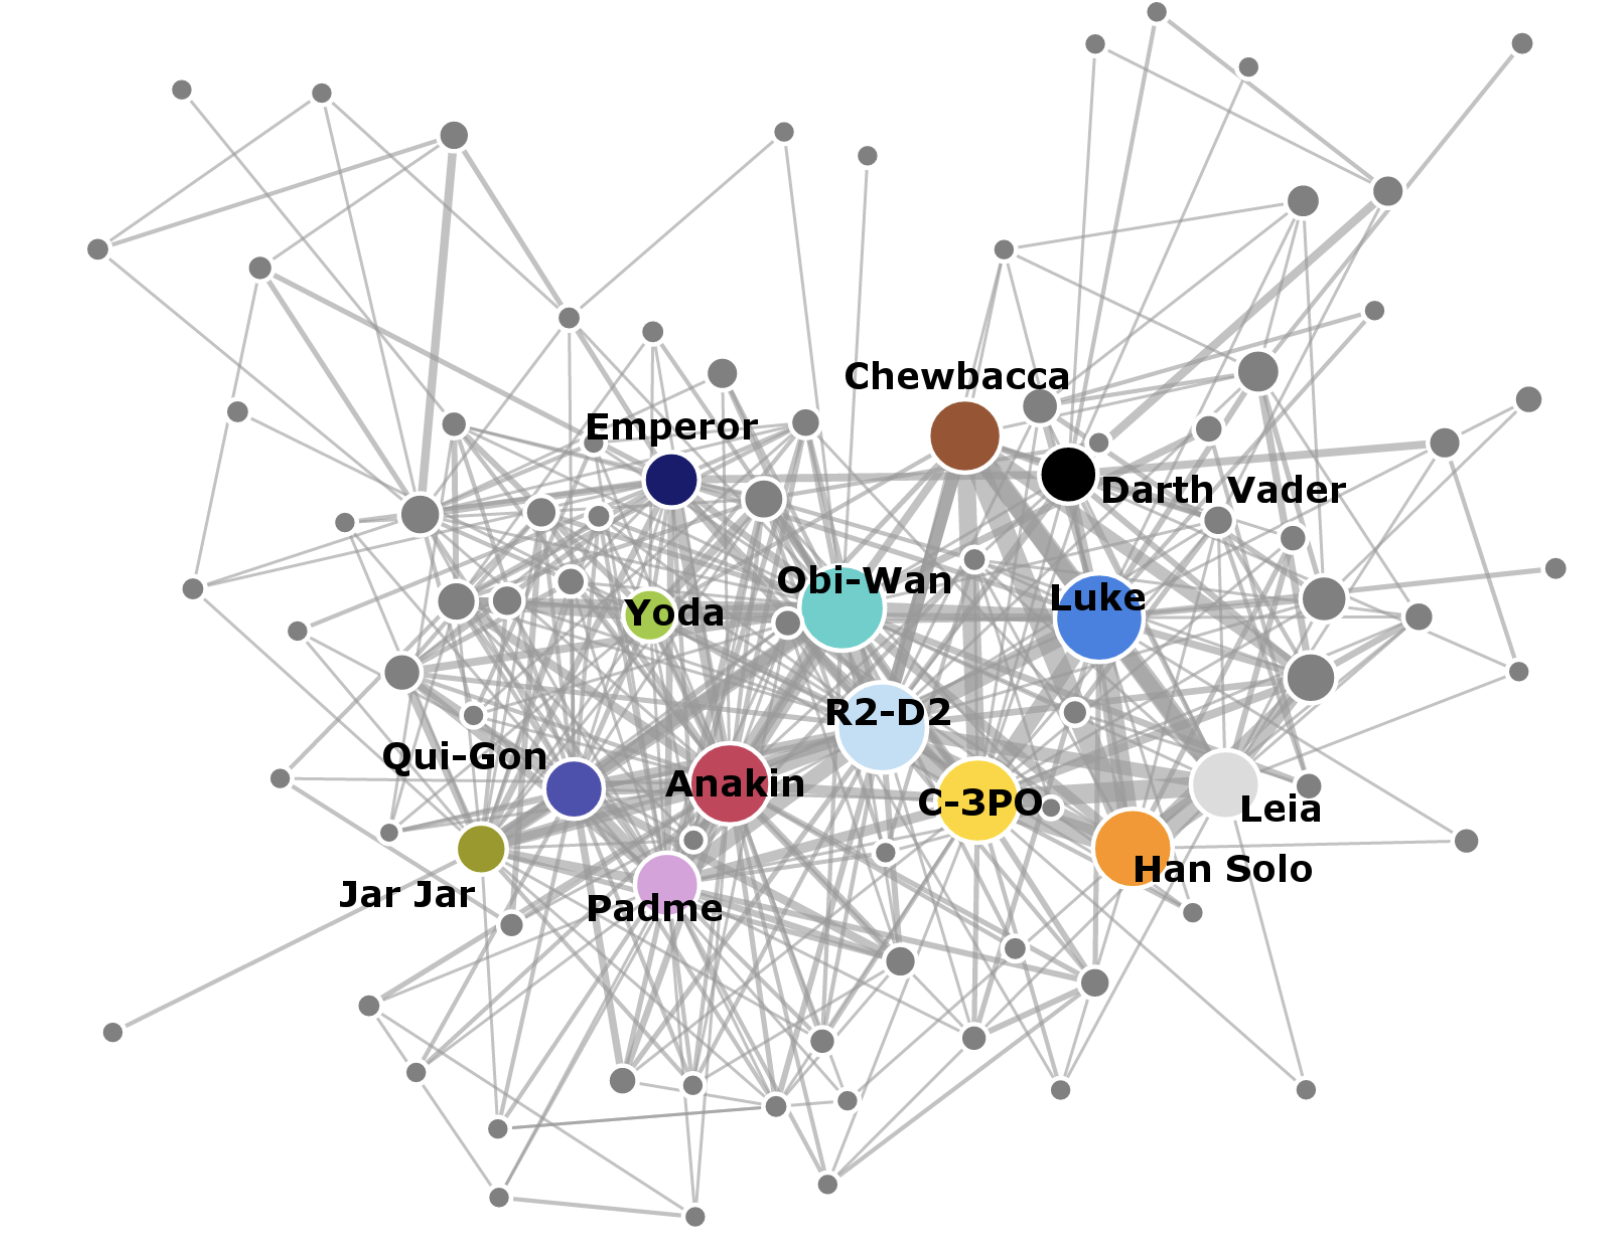
\includegraphics[scale=0.5]{graph-ex.png}
    \caption{An example of the graph of coappearances with major characters labeled.}
    \label{fig: graph}
\end{figure}

There are a few interesting ways to think about clustering this graph, one is that Star Wars is essentially a story about good vs evil, and we should expect the ``good" characters to appear together frequently and the ``bad" characters to appear together frequently, so maybe the graph will seperate in that fashion when we fix $k=2$. Alternatively the series is divided into 3 trilogies, so if we fix $k=3$ maybe we will see primarily characters from episodes 1-3 in one cluster, episodes 4-6 in another, and episode 7 in the last. Higher numbers of clusters may not have a great prior understanding but provide insight into the structure of the films all the same.

\subsubsection*{The $K=2$ Case}

Fixing $K=2$ the major division seems to be between characters from the first three episodes and the remaining 4 films.

The first group contains the main characters from the original trilogy and Episode 7: C-3P0, Luke, Leia, Han, Lando, Poe, Kylo Ren, Finn, Rey, Snoke, BB-8, and many more minor characters from the same: Wedge, Red Leader, Gold Leader, Captain Phasma, General Hux, Maz, etc.

The second group is clearly centered around the prequels (episodes 1-3): Obi-Wan, Qui-Gon, Jar Jar, Greedo, Anakin, Darth Maul, General Grievous, Yoda, Mace Windu, Emperor (Senator Palpatine [spoiler, but it's been out for 15 years]). The major misclassification here is Darth Vader who I would have guessed is a character from episodes 4-6 but gets classified into the group primarily represented by episodes 1-3, but overall the graph seems to split this way.

\subsubsection*{The $K=3$ Case}

This is the case that I think provides the greatest interest into the structure of the data. This really just subsets the $K=2$ case, where now we have a nearly identical group representing characters from episodes 1-3, then a group representing characters from episodes 4-6 and the `good' characters from Episode 7.
The final group is the `bad' characters from Episode 7: Kylo Ren, Captain Phasma, Snoke, General Hux, and other minor characters.


\subsubsection*{The $K=4$ Case}

Like going from $k=2$ to $k=3$, when we increase again we fill the fourth group with a small subset: the rebel pilots from a scene in Episode 7. This contains Yolo Ziff, Ello Asty, and Niv Lek, three characters I had to look up, but all appear in the same role in the same scene with minor parts, so although this may be unexpected, it is a natural way to separate the data.


\subsection*{Code}
\lstset{language=Python}
\footnotesize
\textbf{Main Runner Script}
\begin{lstlisting}
import math
import numpy as np
import sys
sys.path.append("/Users/greg/Google Drive/Spring 19/CS6241/graph-clustering/spectral-clustering/")
from spectral_clustering import *
sys.path.append("/Users/greg/Google Drive/Spring 19/CS6241/graph-clustering/data/")
from read_star_wars import read_star_wars

def main():
    # np.random.seed(416)
    np.random.seed(8818)
    adj_mat, nodes = read_star_wars()
    n_clust = 7
    adj_mat.shape

    # run with homemade k means ##
    node_list, clusters = cluster(adj_mat, n_clust, normalized=True)
    groups = np.array([n.centroid for n in node_list])
    # print([n.pos for n in node_list])
    # groups
    for clust in range(n_clust):
        inds = np.where(groups == clust)
        print("GROUP:")
        [print(nodes[ii]) for ii in list(inds[0])]
        print("\n\n")

if __name__ == '__main__':
    main()
\end{lstlisting}

\textbf{Spectral Clustering}
\begin{lstlisting}
import math
import numpy as np
from scipy.cluster.vq import kmeans2
import matplotlib.pyplot as plt
import sys
from k_means import kmeans


def degree_matrix(W):
    """
    takes in adjacency matrix and returns the diagonal of the
    corresponding degree degree matrix
    """

    return np.sum(W, axis=1)

def laplacian_first_evecs(A, n_cluster, normalized=False):
    """
    computes the graph laplacian from an adjacency matrix
    """
    D = np.diag(degree_matrix(A))
    # print(1/np.diag(D))
    L = D - A

    if normalized:
        sqrt_inv_D = np.diag(np.diag(D)**(-0.5))
        # print(np.matmul(sqrt_inv_D, sqrt_inv_D))
        L = np.matmul(np.matmul(sqrt_inv_D, L), sqrt_inv_D)

    w, v = np.linalg.eig(L)
    v = v[:, :n_cluster]
    if normalized:
        v = np.matmul(sqrt_inv_D, v)
    return v


def cluster(A, n_cluster=5, normalized=False):
    V = laplacian_first_evecs(A, n_cluster, normalized)
    # U = first_evecs(L, n_cluster, normalized)
    # return U
    # print(V.shape)
    # clusters = kmeans2(V, n_cluster, iter=20000)
    clusters = kmeans(V, n_cluster, niters=2000)
    return clusters
\end{lstlisting}

\textbf{K-Means}
\begin{lstlisting}
import math
import numpy as np
import matplotlib.pyplot as plt

class node():
    """docstring for node."""
    def __init__(self, pos, original_ind):
        self.pos = pos

        self.label = original_ind
        self.centroid = None

class centroid():
    """docstring for centroid."""
    def __init__(self, pos, id):
        self.pos = pos
        self.id = id


def get_dist(node, centroid):
    return np.linalg.norm(node.pos - centroid.pos)

def compute_new_center(node_positions):
    avg_pos = np.mean(node_positions, 0)
    return avg_pos


def update_assignments(node_list, centroids):
    ## look through list and get distances to all centroids for all nodes ##
    for node in node_list:
        min_dist = None
        for centroid in centroids:
            dist = get_dist(node, centroid)
            if min_dist is None:
                min_dist = dist
                node.centroid = centroid.id
            elif dist < min_dist:
                min_dist = dist
                node.centroid = centroid.id

    return node_list


def update_centroid_centers(node_list, centroids):
    # print("n centr = ", len(centroids))
    for centroid in centroids:
        has_node = False
        # just a temporary place holder #
        node_positions = centroid.pos
        for node in node_list:
            if node.centroid == centroid.id:
                has_node = True
                node_positions = np.vstack((node_positions, node.pos))

        # only update if there are any nodes in the centroid #
        if has_node:
            centroid.pos = compute_new_center(node_positions[1:, ])

    return centroids

def kmeans(node_mat, n_clusters, niters=100):
    ## set up everything ##
    n_dim = node_mat.shape[1]

    # random centroids #
    start_centers = np.random.rand(n_clusters, n_dim)*0.1 - 0.05
    centroids = [centroid(start_centers[ii, :], ii) for ii in range(n_clusters)]
    # node list #
    node_list = []
    for rr in range(node_mat.shape[0]):
        node_list.append(node(node_mat[rr, :], rr))

    for ii in range(niters):
        node_list = update_assignments(node_list, centroids)
        centroids = update_centroid_centers(node_list, centroids)

    return node_list, centroids
\end{lstlisting}

\textbf{Read Data}
\begin{lstlisting}
import json
import numpy as np
import math
import sys
sys.path.append("../")

def read_star_wars():
    fpath = "/Users/greg/Google Drive/Spring 19/CS6241/graph-clustering/data/"
    fname = "star_wars_clean.json"

    ## BAD NODE = 76 ##
    with open(fpath+fname) as f:
        data = json.load(f)
        nodes = data['nodes']
        edges = data['links']

    # nodes[76]
    n_nodes = len(nodes)
    adj_mat = np.zeros((n_nodes, n_nodes))

    ## refactor edges ##
    for edge in edges:
        if edge['source'] > 76:
            edge['source'] -= 1
        if edge['target'] > 76:
            edge['target'] -= 1


    for edge in edges:
        adj_mat[edge['source'], edge['target']] = edge['value']
        adj_mat[edge['target'], edge['source']] = edge['value']

    nodes = [node['name'] for node in nodes]

    return adj_mat, nodes
\end{lstlisting}
\nocite{*}
\bibliography{main}
\bibliographystyle{plain}
\end{document}
